% Gemini theme
% https://github.com/anishathalye/gemini

\documentclass[final]{beamer}

% ====================
% Packages
% ====================

\usepackage[T1]{fontenc}
\usepackage{lmodern}
\usepackage[size=a0]{beamerposter}
\usetheme{gemini}
\usecolortheme{mit}
\usepackage{graphicx}
\graphicspath{{./img/}}
\usepackage{epstopdf}
\usepackage[backend=bibtex,style=phys,sorting=nyt]{biblatex} % Use style=draft for troubleshooting.
\addbibresource{references.bib}

% ====================
% Lengths
% ====================

% If you have N columns, choose \sepwidth and \colwidth such that
% (N+1)*\sepwidth + N*\colwidth = \paperwidth
\newlength{\sepwidth}
\newlength{\colwidth}
\setlength{\sepwidth}{0.025\paperwidth}
\setlength{\colwidth}{0.3\paperwidth}

\newcommand{\separatorcolumn}{\begin{column}{\sepwidth}\end{column}}

% ====================
% Title
% ====================

\title{Deep Stacking of AGN Hypervariables}

\author{Alexander S. Wheaton \inst{1}}

\institute[shortinst]{\inst{1} The University of Edinburgh}

% ====================
% Footer (optional)
% ====================

\footercontent{
  \href{https://www.github.com/lt-stacking-project}{https://www.github.com/lt-stacking-project} \hfill
  \href{mailto:s1572046@ed.ac.uk}{s1572046@ed.ac.uk}}
% (can be left out to remove footer)

% ====================
% Logo (optional)
% ====================

% use this to include logos on the left and/or right side of the header:
\logoright{\includegraphics[height=7cm]{crest.eps}}
% \logoleft{\includegraphics[height=7cm]{logo2.pdf}}

% ====================
% Body
% ====================

\begin{document}

\begin{frame}[t]
\begin{columns}[t]
\separatorcolumn

\begin{column}{\colwidth}

\begin{block}{\LARGE Gaussian Fits on J094511}
\begin{figure}[t]
    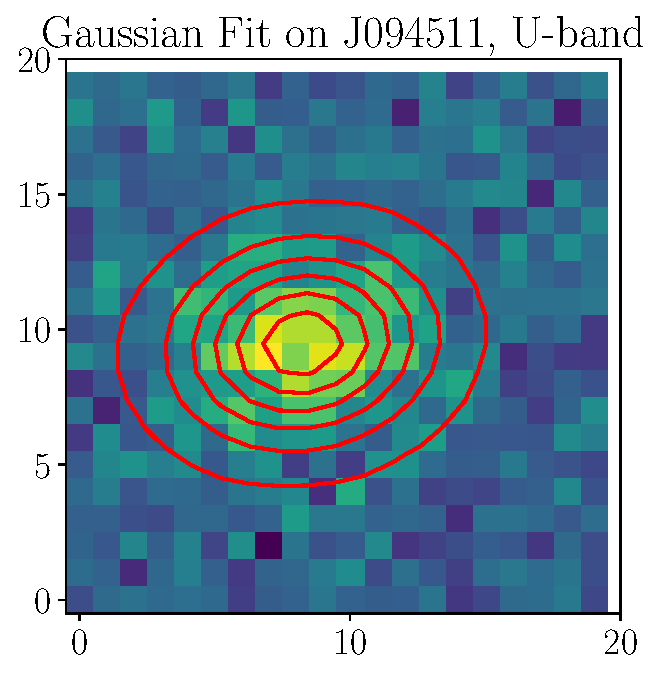
\includegraphics[width=0.32\textwidth]{gauss_fit_wcs_U_stack.eps}
    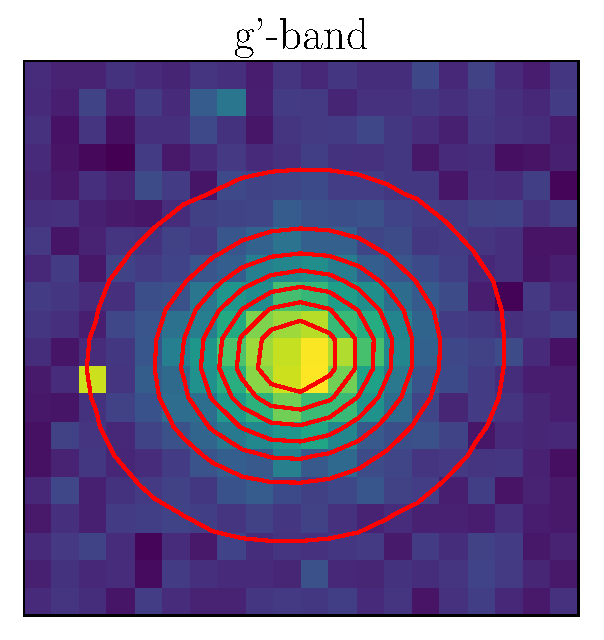
\includegraphics[width=0.32\textwidth]{gauss_fit_wcs_G_stack.eps}
    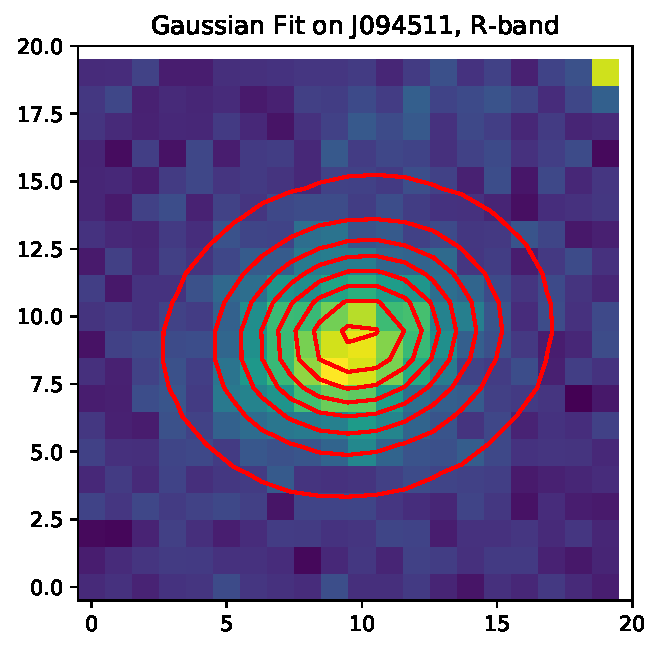
\includegraphics[width=0.32\textwidth]{gauss_fit_wcs_R_stack.eps}
    \caption{\Large Gaussian fit on J094511 in the Sloan $u'g'r'$ bands.}
    \label{fig:gauss_fit_wcs_stack}
\end{figure}
\end{block}

\begin{block}{\LARGE A Faint Intervening Galaxy?}
\Large If the AGN is modeled as point source and intervening star modeled as a lens (simple microlensing model), it is possible to compute the lightcurve $F(t) = \mu(t)F_s$ which describes the evolution of the lensed AGN with respect to its unlensed flux, as described by Bruce et al. (2017).\cite{bruce_2017} If there is a diffuse but faint intervening source, there should be a flux contribution $F_b$ from this source, measurable in the profile of J094511.

Extracting this profile from the existing Liverpool Telescope (LT) data is challenging. The object is very faint, with a low object to sky background ratio. Stacking many frames from the LT increases the signal to noise (S/N) ratio, but they must first be aligned.
\end{block}

\begin{alertblock}{\LARGE WCS Alignment and Stacking}

\Large Using the World Coordinate System (WCS) data stored in FITS file headers, I have devised an algorithmic way to centroid on any object in a FITS file by specifying its known equatorial coordinates. Individual frames are then aligned to this point and stacked to increase the S/N ratio on that object. Once stacked, we can fit a Gaussian function to the resulting data to quantify the profile of the object (see Fig. \ref{fig:gauss_fit_wcs_stack}).
\newline
\begin{table}[h!]
    \centering
    \begin{tabular}{| c | c | c | c | c | c | c |} \hline
        Band & Amplitude & $x_0$ & $y_0$ & $\sigma_x$ & $\sigma_y$ & $\theta$ \\ \hline \hline
        $u'$ & $250(10)$ & $8.2(2)$ & $9.5(1)$ & $0.83(4)''$ & $0.64(3)''$ & $0.2(1)$ \\
        $g'$ & $2170(50)$ & $9.34(6)$ & $8.85(5)$ & $0.75(2)''$ & $0.66(2)''$ & $0.2(1)$  \\
        $r'$ & $2270(60)$ & $9.37(7)$ & $8.81(6)$ & $0.75(2)''$ & $0.60(2)''$ & $0.02(1)$ \\ \hline
    \end{tabular}
    \caption{\Large Fitted Gaussian parameters for WCS based stacking.}
    \label{tab:wcs_gaussians}
\end{table}
This method, however, is limited to whole pixel resolution, and introduces several systematic uncertainties.
\end{alertblock}

\end{column}

\separatorcolumn

\begin{column}{\colwidth}

\begin{alertblock}{\LARGE Abstract}
In this project, I examine the unusual luminosity of the galactic nucleus
SDSS J094511 located at redshift $z=0.758$ using data gathered with the
Liverpool Telescope on Las Palmas between 2012 and 2018. I develop several
algorithms for centroiding on the object, for resampling to obtain higher
resolution, and for stacking images to increase the S/N ratio in the frame.
I extract radial and linear cross sections from the object and compare these
to the point-spread-function of the Liverpool Telescope CCD to corroborate
the hypothesis that linear increases in the luminosity over large timescales
are \textit{not} due to instability of the viscous AGN accretion disk, but a
gravitational microlensing event by a star in an intervening galaxy or dwarf
galaxy.
\end{alertblock}

\begin{block}{\LARGE What are Hypervariable AGN?}
\Large Active galactic nuclei (AGN) are variably luminous, deep sky objects. The source of their luminosity is widely believed to be the accretion of matter into a disk around supermassive black holes.\cite{lawrence_2018} The accretion disk model explains many of their observed properties, including:

\begin{center}
\begin{itemize}
    \centering
    \item \textbf{Luminous and compact appearance}
    \item \textbf{Broad spectrum energy emission}
    \item \textbf{Variable over short timescales}
\end{itemize}
\end{center}

But Lawrence et al. (2016) identify several slowly evolving, blue ``hypervariable'' AGN, which increase and decrease smoothly by several magnitudes over a period of years. One such hypervariable AGN is SDSS J094511. These are not compatible with the AGN accretion disk model, and they propose that gravitational lensing events are responsible for variable luminosity in these objects.\cite{lawrence_2016}
\end{block}

\begin{block}{\LARGE Radial Profiles of J094511}
\begin{figure}[h!]
    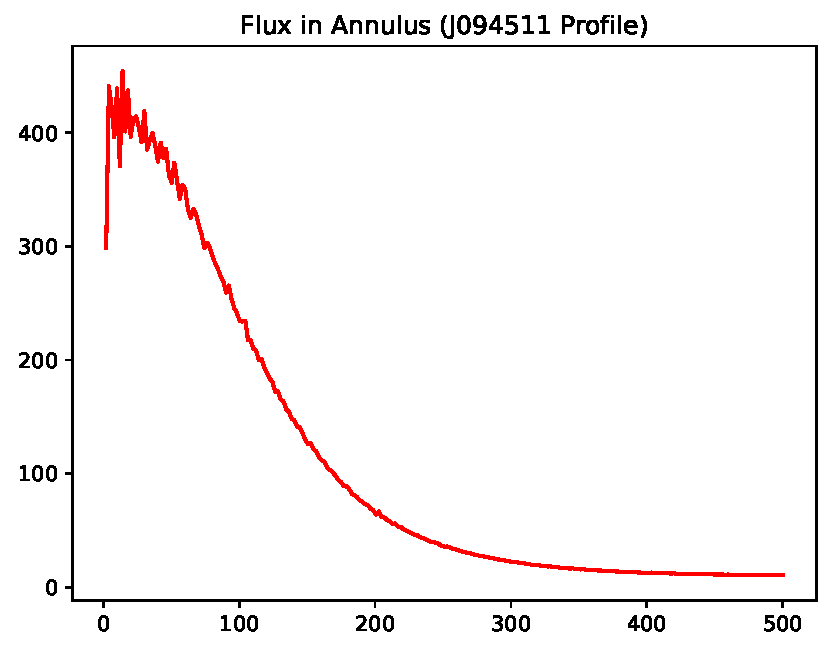
\includegraphics[width=0.32\textwidth]{J094511_U_annulus_flux.eps}
    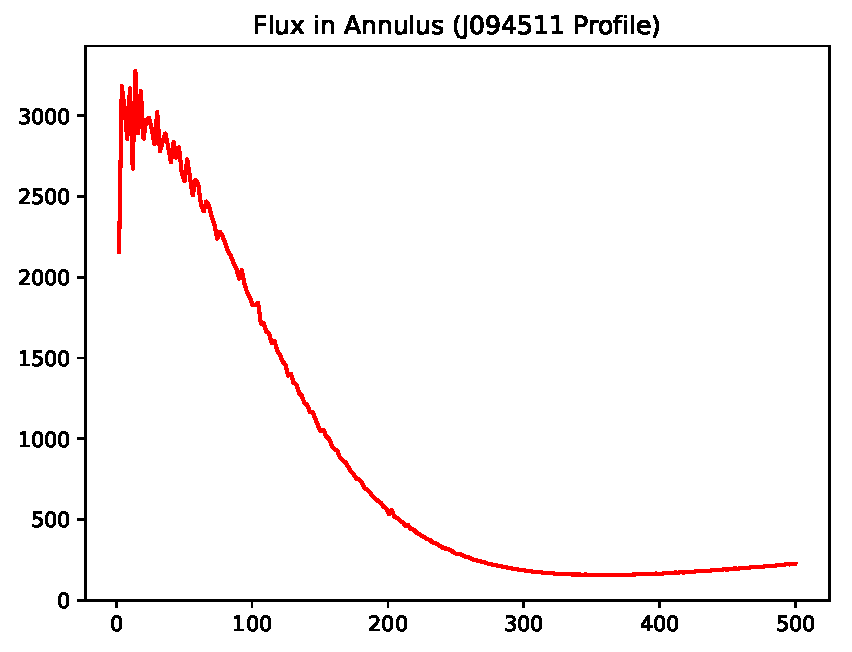
\includegraphics[width=0.32\textwidth]{J094511_G_annulus_flux.eps}
    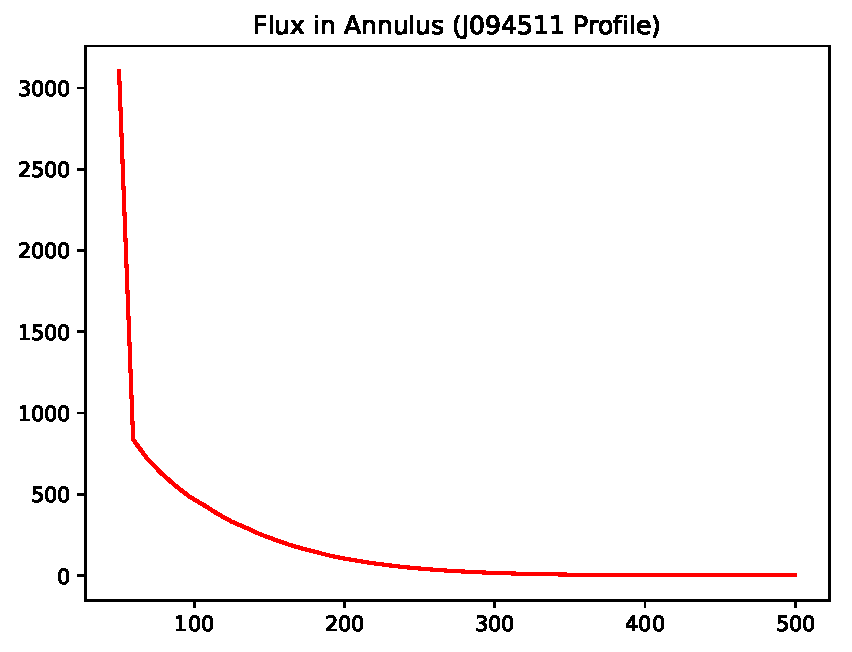
\includegraphics[width=0.32\textwidth]{J094511_R_annulus_flux.eps}
    \caption{\Large Radial profile of J094511 in the Sloan $u'g'r'$ bands.}
    \label{fig:radial_profiles}
\end{figure}

\Large The radial profiles of J094511 are Gaussian in form. By training the algorithm an intragralactic point source, it is possible to obtain the point-spread-function (PSF) response of the LT, and subtract this from the profile of J094511 to obtain a profile of the intervening galaxy, the area integral of which is $F_b$.
\end{block}

\end{column}
\separatorcolumn
\begin{column}{\colwidth}

\begin{block}{\LARGE Gaussian Resampling of J094511}
\begin{figure}[h!]
    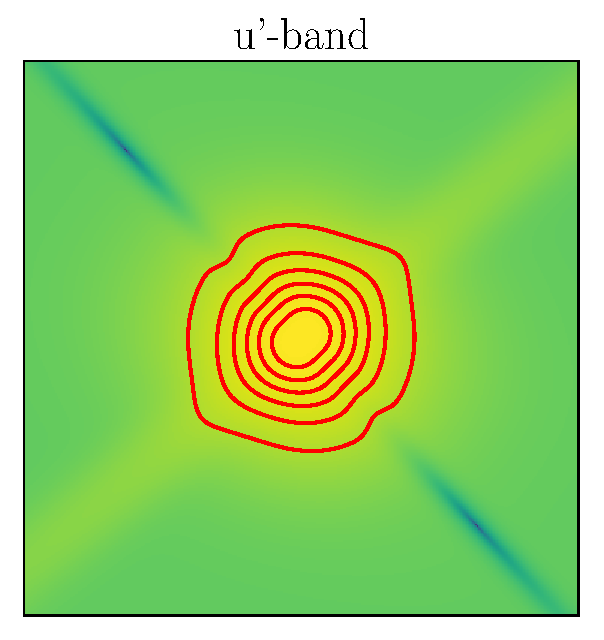
\includegraphics[width=0.32\textwidth]{J094511_U_resampled_stack.eps}
    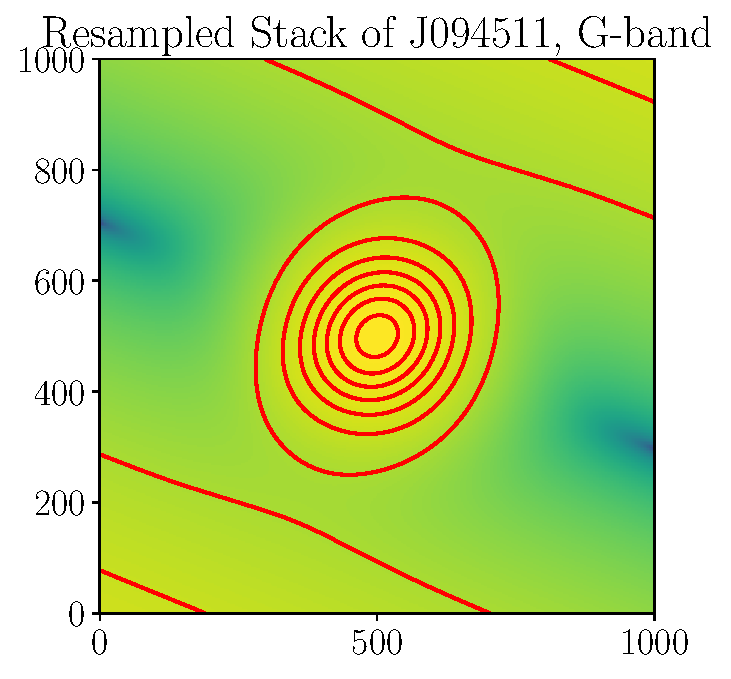
\includegraphics[width=0.32\textwidth]{J094511_G_resampled_stack.eps}
    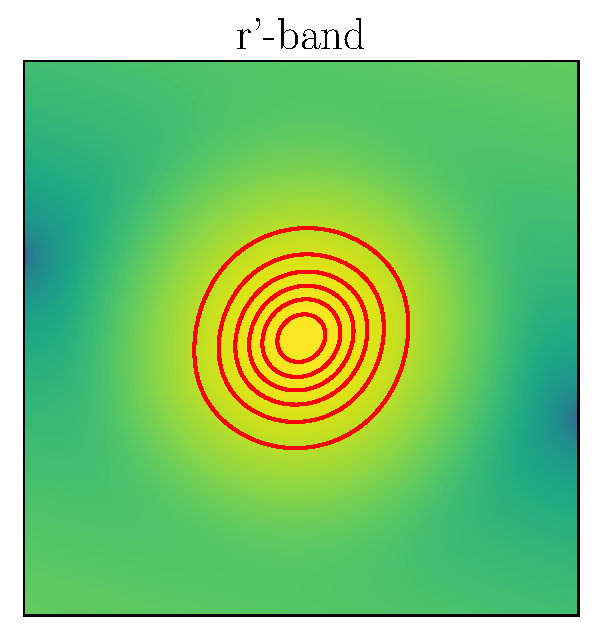
\includegraphics[width=0.32\textwidth]{J094511_R_resampled_stack.eps}
    \caption{\Large Resampled stacks of J094511 in the Sloan $u'g'r'$ bands.}
    \label{fig:resampled_stacks}
\end{figure}
\end{block}

\begin{alertblock}{\LARGE Gaussian Resampling for Higher Resolution}
\Large By fitting a Gaussian function to individual frames, though, we can interpolate the flux at non-integer pixel values. The fitted function has ``infinite'' resolution; and by aligning and summing these fitted forms, we can obtain a high S/N ratio for the object at any desired resolution. Once again, fitting a Gaussian function to the resulting stack allows us to quantify the object profile.
\newline
\begin{table}[h!]
    \centering
    \begin{tabular}{| c | c | c | c | c | c | c |} \hline
        Band & Amplitude & $x_0$ & $y_0$ & $\sigma_x$ & $\sigma_y$ & $\theta$ \\ \hline \hline
        $u'$ & $385.42(5)$ & $499.5$ & $499.5$ & $0.568''$ & $0.525''$ & $0.689$ \\
        $g'$ & $2889.0(2)$ & $499.5$ & $499.5$ & $0.611''$ & $0.557''$ & $3.969$ \\
        $r'$ & $3168.9(2)$ & $499.5$ & $499.5$ & $0.529''$ & $0.579''$ & $2.472$ \\ \hline
    \end{tabular}
    \caption{\Large Fitted Gaussian parameters for resampled stacking.}
    \label{tab:resampled_gaussians}
\end{table}

The parameters in Table \ref{tab:resampled_gaussians} are fitted to a resampled image with 50x the resolution of the LT frames. The uncertainties on these parameters are trivially small, unless listed. Another algorithm was devised to extract the radial profiles in Fig. \ref{fig:radial_profiles} by summing the counts in annuli placed around the object.

All of these algorithms are open source and licensed under GNU GPLv3 License, are free to use, and have wide applications in computational astronomy.
\end{alertblock}

\begin{block}{\small References}
\small
\printbibliography
\end{block}

\end{column}

\separatorcolumn
\end{columns}
\end{frame}

\end{document}
